\documentclass[usenames,dvipsnames]{beamer}
\usetheme{Warsaw}
\usepackage{lmodern}
\usepackage[squaren,Gray]{SIunits}
\usepackage{amsmath}
\usepackage[utf8]{inputenc}

\newcommand{\norm}[1]{\left\lVert#1\right\rVert}


%Information to be included in the title page:
\title{Online Estimation of Inertial Parameters Using a Recursive Total Least-Squares Approach}
\author{François Le Rall}
\institute{Nomagic – Robotic Seminar}
\date{2019}



\begin{document}

\frame{\titlepage}

\begin{frame}{Overview}
 \tableofcontents

\end{frame}


\section{Definition of the problem}

\begin{frame}
 \frametitle{Definition of the problem}

 \begin{minipage}{.5\textwidth}
  \begin{itemize}
   \item F/T sensor Gamma measuring:
         \begin{itemize}
          \item force ${}^S f$,
          \item torque ${}^S \tau$,
          \item in the sensor frame $S$.
         \end{itemize}
   \item Payload grasped by the suction tool:
         \begin{itemize}
          \item mass $m$,
          \item center of mass ${}^S c$,
          \item moment of inertia ${}^S I$,
          \item linear acceleration ${}^S a$,
          \item angular acceleration ${}^S \alpha$,
          \item angular velocity ${}^S \omega$,
          \item gravity ${}^S g$.
         \end{itemize}
  \end{itemize}
 \end{minipage}%
 \begin{minipage}{0.5\textwidth}
  \centering
  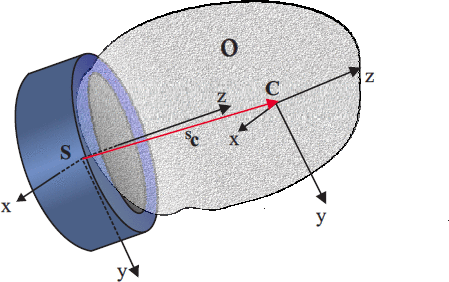
\includegraphics[scale=0.4]{images/scheme.png}
 \end{minipage}

\end{frame}

\begin{frame}
  \frametitle{Definition of the problem}
  \center
  {\Huge \textbf{How to make a reliable online estimation of the weight of the item grasped?}}
\end{frame}

\begin{frame}
 \frametitle{Newton-Euler Approach}

 The motion of the body due to external forces is described by the two equations:

 \begin{align}
  {}^S f    & = m {}^S a - m {}^S g + {}^S \alpha \times m {}^S c + {}^S \omega \times ({}^S \omega \times m {}^S c)           \\
  {}^S \tau & = {}^S I {}^S \alpha + {}^S \omega \times ({}^S I {}^S \omega) + m {}^S c \times {}^S a - m {}^S c \times {}^S g
 \end{align}

 also in matrix form:

 \begin{equation}
  \begin{pmatrix}
   {}^S f    \\
   {}^S \tau
  \end{pmatrix}
  = {}^S A({}^S a, {}^S \alpha, {}^S \omega, {}^S g) {}^S \varphi
 \end{equation}

 with ${}^S \varphi = (m, m {}^S c_x, m {}^S c_y, m {}^S c_z, {}^S I_{xx}, {}^S I_{xy}, {}^S I_{xz}, {}^S I_{yy}, {}^S I_{yz}, {}^S I_{zz}) {}^T$
\end{frame}


\begin{frame}
 \frametitle{Optimisation problem}

 During the motion of the payload, $M$ ${}^S A_{ext}$ matrices are compiled at subsequent instants of time:
 \begin{gather}
  {}^S A_{\Xi} = [{}^S A_1^T {}^S A_2^T \ldots {}^S A_M^T] {}^T \\
  \begin{pmatrix}
   {}^S f    \\
   {}^S \tau
  \end{pmatrix}_{\Xi}
  = \Bigg[\begin{pmatrix}
  {}^S f    \\
  {}^S \tau
  \end{pmatrix}_1^T
  \begin{pmatrix}
   {}^S f    \\
   {}^S \tau
  \end{pmatrix}_2^T
  \ldots \begin{pmatrix}
  {}^S f    \\
  {}^S \tau
  \end{pmatrix}_M^T \Bigg] {}^T
 \end{gather}

 The optimization problem is the following, for every instant of time ($\Xi$ batch of size $M$):

 \begin{align*}
  \underset{{}^S \varphi_M}{\textrm{minimize}} \quad &
  \norm{ \begin{pmatrix}
  {}^S f    \\
  {}^S \tau
  \end{pmatrix}_{\Xi}
  - {}^S A_{\Xi} {}^S \varphi_M } \\
  \textrm{subject \ to} \quad & m_M \geq 0   \\
                              & c_{zM} \geq 0
 \end{align*}

\end{frame}

\section{Estimation of the inertial parameters}
\subsection{Estimation method}


\begin{frame}
 \frametitle{Comparison of different methods}

 \begin{itemize}
  \item Recursive Least-Squares methods
        \begin{itemize}
         \item Error model: $\begin{pmatrix}
               {}^S f    \\
               {}^S \tau
         \end{pmatrix}_{\Xi}
         + e = {}^S A_{\Xi} {}^S \varphi $.
         \item \textcolor{red}{Errors in the data matrix ${}^S A_{\Xi}$ are not considered.}
        \end{itemize}
  \item Recursive Instrumental Variables Method
        \begin{itemize}
         \item \textcolor{ForestGreen}{Yield unbiased estimates in the presence of correlated noise.}
         \item \textcolor{red}{Errors in the data matrix ${}^S A_{\Xi}$ are not considered.}
        \end{itemize}
  \item Recursive Total Least-Squares (RTLS) Method
        \begin{itemize}
         \item \textcolor{ForestGreen}{More appropriate error model: $\begin{pmatrix}
                     {}^S f    \\
                     {}^S \tau
               \end{pmatrix}_{\Xi}
               + e = ({}^S A_{\Xi} + E) {}^S \varphi $.}
         \item \textcolor{red}{Require update of the Singular Value Decomposition (SVD) at each estimation cycle with a complexity $O(mn \min(n, m))$.}
        \end{itemize}
 \end{itemize}
\end{frame}

\begin{frame}
 \frametitle{Recursive Total Least-Squares (RTLS) Method}

 \begin{figure}
  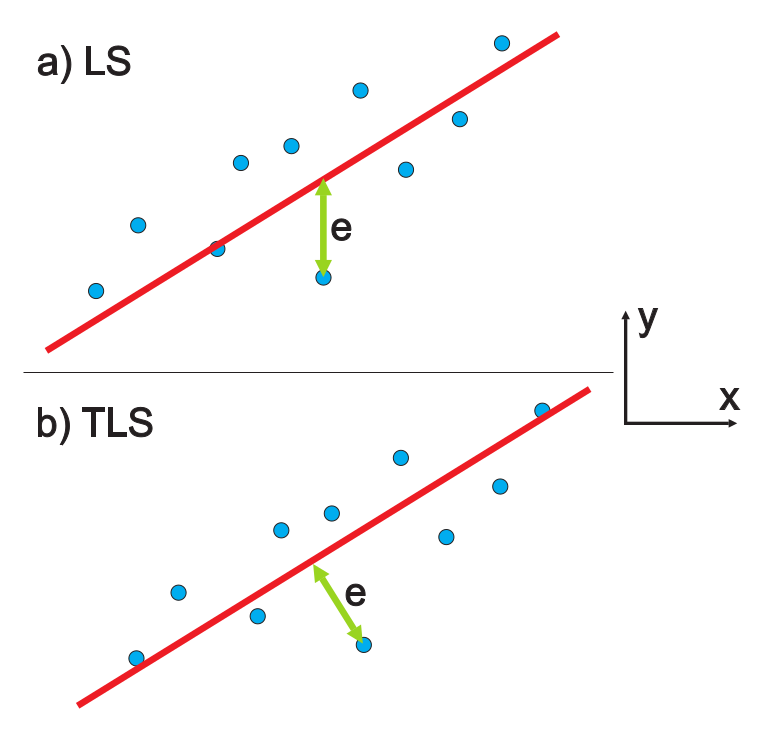
\includegraphics[scale=0.2]{images/LS_vs_TLS.png}
  \caption{In contrast with LS approach, TLS approach considers errors in both x- and y-directions.}
\label{images_vs}
 \end{figure}

\end{frame}


\subsection{Relevance of a recursive least-square algorithm}

\begin{frame}
 \frametitle{Relevance of a recursive least-square algorithm}

\begin{itemize}
  \item The \textit{recursive} least-squares methods seems to be relevant for \textbf{online} estimation of inertial parameters.
  \item The payload can be estimated at the end of the placement move to the item recognition position.
  \item The optimisation problem become:
  \begin{align*}
   \underset{{}^S \varphi}{\textrm{minimize}} \quad &
   \norm{ \begin{pmatrix}
   {}^S f    \\
   {}^S \tau
   \end{pmatrix}_{\Xi}
   - {}^S A_{\Xi} {}^S \varphi } \\
   \textrm{subject \ to} \quad & m \geq 0   \\
                               & c_z \geq 0
  \end{align*}
  \item [$\rightarrow$] \textcolor{RoyalPurple}{Is it necessary to have online update of the inertial parameters?}

\end{itemize}
\end{frame}


\begin{frame}
  \frametitle{My next steps}

  \begin{itemize}
    \item Test a simplified version of the method:
    \begin{itemize}
      \item Least-squares method only
      \item Test on different items and differents trajectories
    \end{itemize}
  \item Test of the recursive total methods:
  \begin{itemize}
    \item Comparison of the running time of each method
  \end{itemize}
  \item Setup performance improvement:
  \begin{itemize}
    \item Estimation of the sensor offsets
    \item Estimation of the sensitivity of ${}^S \varphi$ to error
    \item (wide open for suggestions)
  \end{itemize}
  \end{itemize}
\end{frame}


\section{Performance improvement}
\subsection{Estimation of the sensor offsets}

\begin{frame}
 \frametitle{Estimation of the sensor offsets}
 Strain gage force/torque sensors typically show offsets that would deteriorate the estimation.

 \begin{itemize}
  \item \textcolor{red}{Currently, the sensor is reset every 20/25 iterations (it takes a couple of second)},
  \item \textcolor{ForestGreen}{Directly estimating the sensor offsets}.
 \end{itemize}

 The number of parameters to estimate increase from 10 to 16:
 \begin{gather}
  {}^S \varphi_{ext} = [f_{O_x}, f_{O_y}, f_{O_z}, {}^S \varphi] {}^T \\
  {}^S A_{ext} = [\mathbb{I}_{6 \times 6} {}^S A]
 \end{gather}

 {\footnotesize Drift effects can be neglected since the estimation duration is quite small ($\sim 3 \second$)}
\end{frame}


\subsection{Estimation of the error sensitivity}

\begin{frame}
 \frametitle{Estimation of the sensitivity of ${}^S \varphi$ to error}

 Considering the correlation matrix $\Upsilon$ consisting of $M$ ${}^S A$ matrices\footnote{The correlation matrix should be computed with the experimental joint angle setpoints.}:

 \begin{equation}
  \Upsilon = {}^S A_{\Xi}^T {}^S A_{\Xi}
 \end{equation}

 The sensitivity of ${}^S \varphi$ to error can be shown to increase with the condition number\footnote{The condition number of a function measures how much the output value of the function can change for a small change in the input argument: $\lim_{\varepsilon \rightarrow 0} \sup _{\|\delta x \|\ \leq \varepsilon} \| \delta f \| ^{}/ \| \delta x \|$ } $\kappa(\Upsilon)$.

\end{frame}

\section{Details of the Recursive Total Least-Squares Method}

\begin{frame}
 \frametitle{Recursive Total Least-Squares (RTLS) Method}

 Basic steps:

 \begin{enumerate}
  \item Calculate an initial SVD with a standard SVD algorithm for a small number of data matrix.
  \item Compile a new input matrix consisting of the current data matrix ${}^S A$ and force-torque vector $({}^S f, {}^S \tau ) {}^T$ and perform an SVD update incorporating the new data.
  \item Update estimate: If the deviation between the smallest singular values is less than $\varepsilon$, transform left singular vectors; compute TLS solution from the left singular vectors.
  \item Continue with 2 or stop estimation.
\end{enumerate}

\end{frame}

\begin{frame}
 \frametitle{References}

 \begin{itemize}
  \item [2007] On-line rigid object recognition and pose estimation based on inertial parameters (D. Kubus, T. Kroger)
  \item [2008] On-Line Estimation of Inertial Parameters Using a Recursive Total Least-Squares Approach (D. Kubus, T. Kroger)
  \item [2014] Combining visual and inertial features for efficient grasping and bin-picking (D. Kubus, I. Weidauer)
  \item [2018] Real-Time Identification of Robot Payload using a Multirate Quaternion-based Kalman Filter and Recursive Total Least-Squares (S. Farsoni, C. Talignani Landi)

 \end{itemize}
\end{frame}

\end{document}
